\documentclass[12pt,a4paper]{report}
\usepackage[utf8]{inputenc}
\usepackage{amsmath}
\usepackage{graphicx}
\usepackage{amsfonts}
\usepackage{amssymb}
\author{Frederik Appel Vardinghus-Nielsen}
\begin{document}
\noindent{\Huge Basics of probability}\\\\
Define
\begin{itemize}
\setlength\itemsep{0em}
\item (Event)
\item Axioms of probability
\item Conditional probability
\end{itemize}
Prove
\begin{itemize}
\setlength\itemsep{0em}
\item Law of Total Probability
\item Bayes' Formula
\end{itemize}
\textbf{Definition 1.2 (Event)}. A subset of $S$, $A\subseteq S$, is called an $event$.\\\\
\noindent \textbf{Definition 1.3 (Axioms of Probability)}. A $probability$ $measure$ is a function $P$, which assigns to each event $A$ a number $P(A)$ satisfying
\begin{itemize}
\item \textbf{(a)} $0\leq P(A) \leq 1$
\item \textbf{(b)} $P(S)=1$
\item \textbf{(c)} If $A_1,A_2,\ldots$ is a sequence of $pairwise$ $disjoint$ event, that is, if $i\neq j$, then $A_i\cap A_j=\emptyset$, then
\begin{equation}
P\left(\cup_{k=1}^{\infty}A_k\right)=\sum_{k=1}^{\infty}P(A_k)
\end{equation}
\end{itemize}
\begin{figure}[H]
\centering
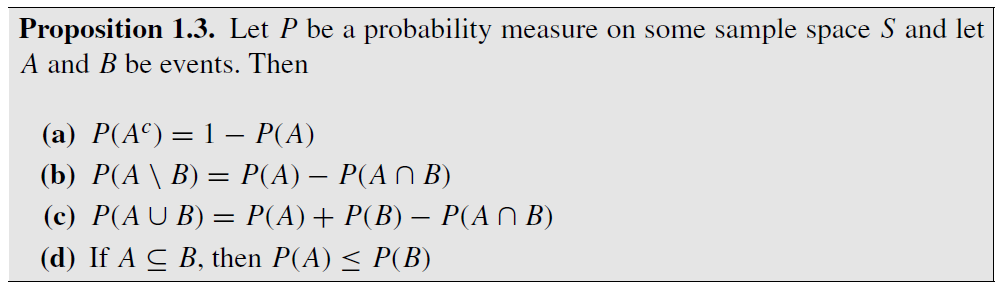
\includegraphics[width=\textwidth]{figures/regneregler.png}
\end{figure}
\begin{figure}[H]
\centering
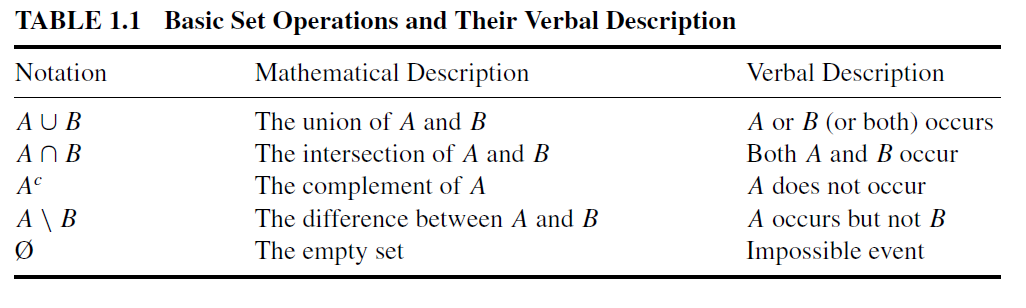
\includegraphics[width=\textwidth]{figures/begreber.png}
\end{figure}
\begin{figure}[H]
\centering
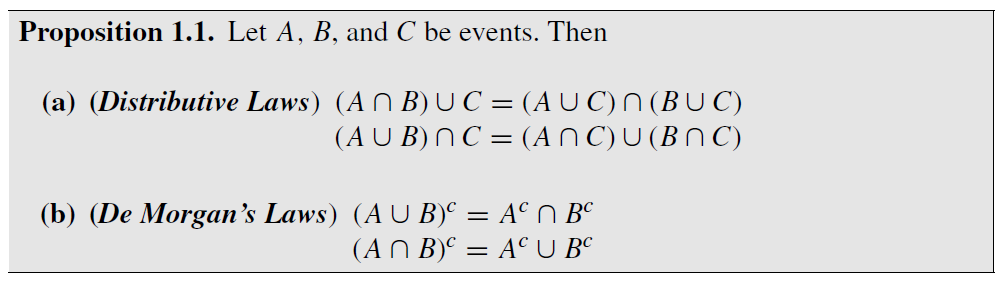
\includegraphics[width=\textwidth]{figures/demorgan.png}
\end{figure}
\begin{figure}
\centering
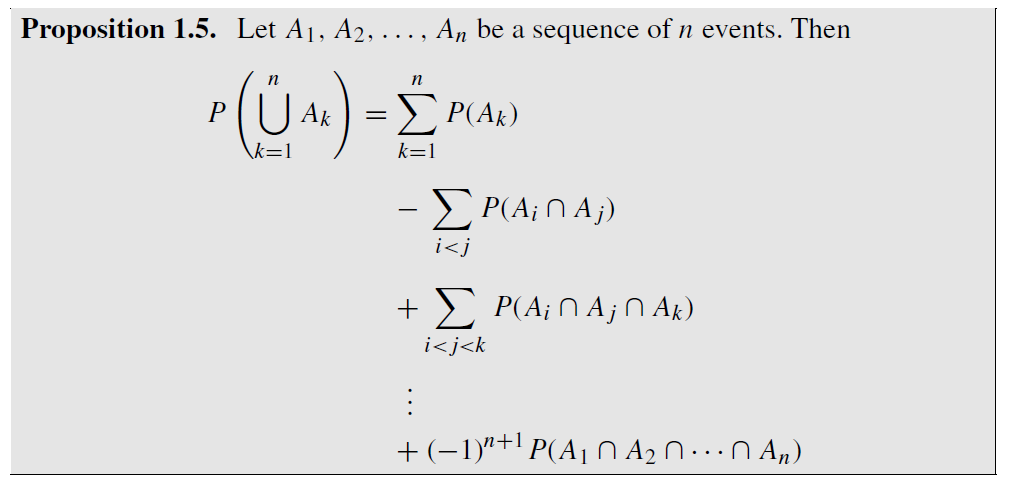
\includegraphics[width=\textwidth]{figures/inc-exc.png}
\end{figure}
\begin{figure}
\centering
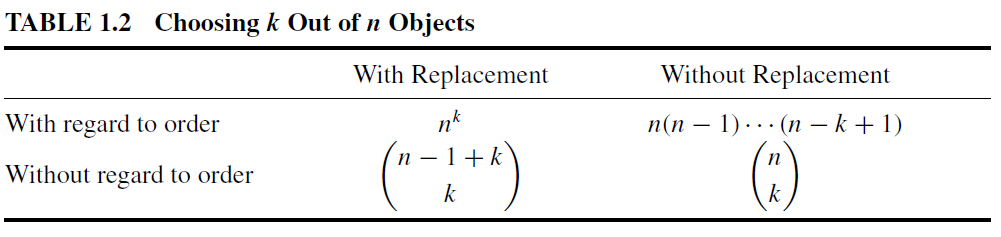
\includegraphics[width=\textwidth]{figures/choosing_skema.png}
\end{figure}
\textbf{Definition 1.4. (Conditional probability).} Let $B$ be an event such that $P(B)>0$. For any event $A$, denote and define the $conditional$ $probability$ $of$ $A$ $given$ $B$ as
\begin{equation}
P(A|B)=\frac{P(A\cap B)}{P(B)}
\end{equation}
\textbf{Theorem 1.1 (Law of Total Probability).} Let $B_1,B_2,\ldots$ be a sequence of events such that
\begin{itemize}
\item[] \textbf{(a)} $P(B_x)>0$ for $k=1,2,\ldots$
\item[] \textbf{(b)} $B_i$ and $B_j$ are disjoint whenever $i\neq j$
\item[] \textbf{(c)} $S=\cup_{k=1}^{\infty}B_k$
\end{itemize}
Then, for any event $A$, we have
\begin{equation}
P(A)=\sum_{k=1}^{\infty}P(A|B_k)P(B_k)
\end{equation}
\textbf{Bevis}\\
Ved den distibutive lov for uendelige fællesmængder fås
\begin{equation}
A=A\cap B=\cup_{k=1}^{\infty}(A\cap B_k)
\end{equation}
Siden $A\cap B_1,A\cap B_2,\ldots$ er parvis disjunkte og derfor kan summeres fås
\begin{equation}
P(A)=\sum_{k=1}^{\infty}P(A\cap B_k)=\sum_{k=1}^{\infty}P(A|B_k)P(B_k)
\end{equation}
\textbf{Proposition 1.11 (Bayes' Formula).} Under the same assumptions as in the law of total probability and if $P(A)>0$, then for any event $B_j$, we have
\begin{equation}
P(B_j|A)=\frac{P(A|B_j)P(B_j)}{\sum_{k=1}^{\infty}P(A|B_k)P(B_k)}
\end{equation}
\textbf{Bevis}\\
Fra loven om samlet sandsynlighed (law of total probability) kan nævneren skrives om, således
\begin{equation}
P(B_j|A)=\frac{P(A|B_j)P(B_j)}{P(A)}
\end{equation}
som kan omskrives til
\begin{equation}
P(B_j|A)P(A)=P(A|B_j)P(B_j)
\end{equation}
Dette er sandt, da loven om betinget sandsynlighed giver, at de to udtryk er ens.












\end{document}